\section{Overview}
A system architecture is introduced to ease maintenance and ensure scalability.
The architecture consists of four macro components and a database, as can be seen in \Cref{fig:architecture}. The macro components are: Shared, Location Service, Model Agent, and Web Service.

\begin{figure}[H]
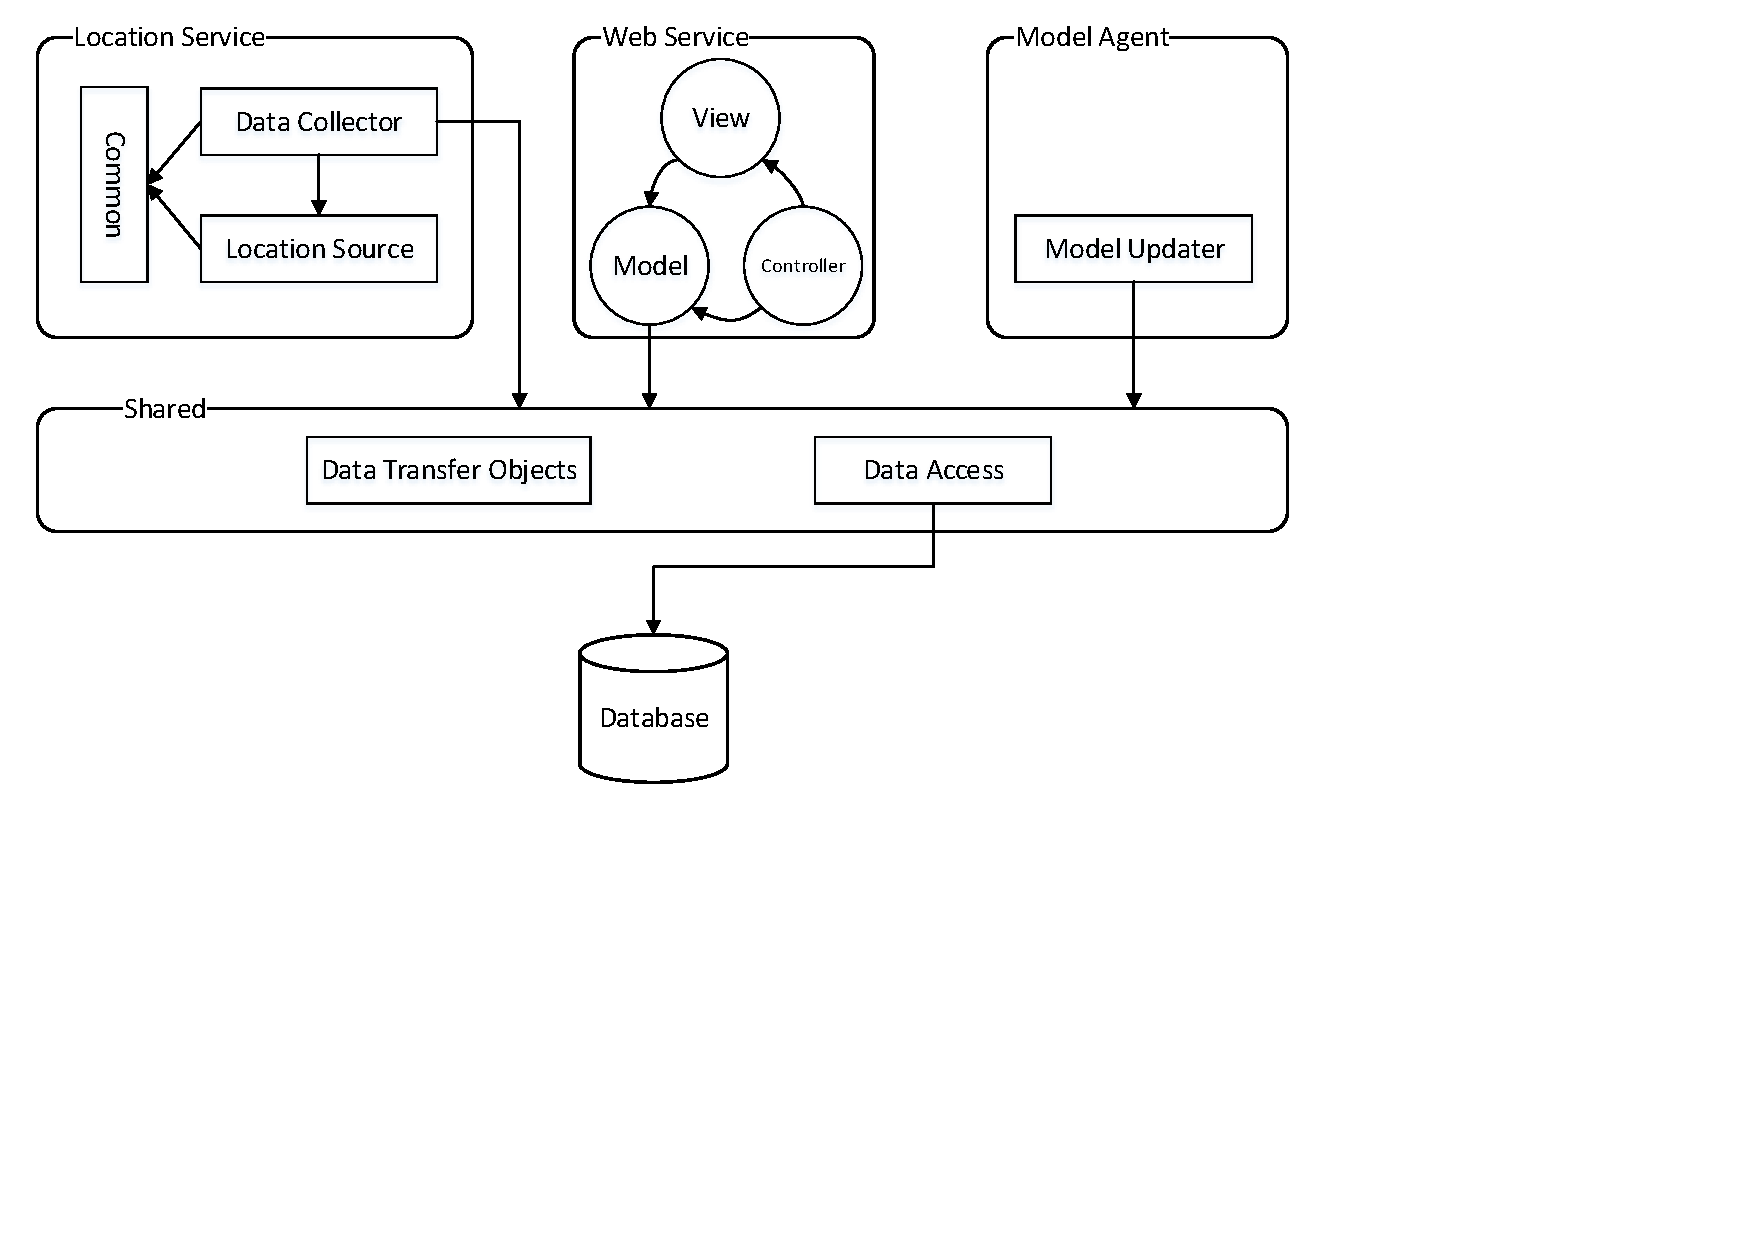
\includegraphics[width=\textwidth, trim={2cm 1cm 6cm 0}]{systemArchitecture.pdf}
\caption{The architecture of the system}
\label{fig:architecture}
\end{figure}
\bruno{What is the difference between a square and circle? Is this maybe confusing?}
\alexander{Maybe use rectangles instead of circles for model, view, controller?}


\subsection{Database} The database used is a MySQL database, and is where all our data is stored.
The design of the database can be found in \Cref{database_design}.


\subsection{Shared}\texttt{Shared} is the macro component containing the \texttt{Data Access} layer and the \texttt{Data Transfer Object} layer.
The macro component's task is to provide extended capabilities to all other macro components.

\paragraph{The Data Access layer} All SQL statements and communication with the database are encapsulated here providing the upper layers a communication protocol to the database.

\paragraph{The Data Transfer Object layer} contains all the shared data types and their attributes, making it possible for all the macro components to treat the data uniformly.


\subsection{Location Service} 
The location service component processes and stores location data directly from a data source. 
The \texttt{Location Service} consists of a \texttt{Location Source} which provides data points to the \texttt{Data Collector}.

\paragraph{The Location Source layer} fetches data from the data source then adapts and casts the data to the appropriate data type in the \texttt{Common} layer.
It is structured so that the \texttt{Location Source} layer can easily be replaced with another source of data.

\paragraph{The Data Collector layer} gathers the data from the \texttt{Location Source} layer and processes it. 
The data is then stored through the \texttt{Data Access} layer.


\subsection{Model Agent}
\texttt{Model Agent}\footnote{An agent is defined as a program that invoke a given task, when a condition is satisfied, then returning to a sleeping state, until the condition is satisfied again.\cite{definitionagent}} is the macro component containing the \texttt{Model Updater} layer.
The macro component's task is to generate and update the model in the system. 

\paragraph{The Model Updater layer} handles the calculation and generation of the models.
The generation of the model works as follows:
Clusters are created based on the GPS data in the database \Cref{clustering:DBSCAN}.
The convex hull of the clusters is calculated and saved as the hotspots of the model.
Markov chains are now created with these clusters as states \Cref{sec:generatemarkov}.

\subsection{Web Service}\label{arch:webservice}
\texttt{Web Service} is the macro component containing the \texttt{Model}, \texttt{View}, and \texttt{Controller}.
The task of the macro component is to provide a web service for users to interact with the system. (see \Cref{chap:webservice})

\paragraph{The Model} manages the application domain and handles data and actions possible for each data type.

\paragraph{The View} manages the display of the \texttt{Model}.

\paragraph{The Controller} handles the user interaction. Based on the user request, the \texttt{Controller} sends commands to the \texttt{Model} and \texttt{View}.